\section{Visual Object Tracking}
\label{sec:VisualObjectTracking}

In this section, we will focus on the \emph{main topic} of this thesis: \textbf{tracking objects visually}. For simplicity, we will first introduce works within the single object tracking category. Section~\ref{sec:MultiObjectTracking} will continue with multiple object tracking.

Many research activities have been devoted to dealing with tracking of objects where visual input is the only information a model is provided with. Since the field of computer vision as a whole has transitioned from manual feature engineering in combination with shallow machine learning algorithms to using deep neural networks in end-to-end style, \gls{vot} as a subfield is no exception. We are going to discuss primarily \gls{sota} approaches, and if we do mention older, maybe even obsolete methods, it will be only for the sake of reference and historical motivation. Furthermore, unless stated otherwise, we will assume a general object tracking model.

\subsection{Initial Deep Learning-Based Solutions}
\label{ssec:InitialDeepLearningBasedSolutions}

At a time of publishing~\cite{held2016goturn}, most generic object trackers required online training from scratch, without taking advantage of available datasets to at least provide a starting point by initial offline training. This was the incentive behind development of the famous \gls{goturn}~\cite{held2016goturn}. This approach used to be \gls{sota} in single object tracking, but nowadays it is considered obsolete. A major issue is that the object has to be located initially, and occlusion handling is not performed as well as management of abrupt changes in position. So it is common for the object to drift away. Nevertheless, it stands to reason that the notion of leveraging data for offline training has pervaded the \gls{vot} community ever since. Nowadays, it is scarce to find a tracker that is trained online purely from scratch.

Given an initial state in a form of a \gls{bbox} belonging to the first frame (a search region), the network then crops a new region in the next frame and tries to find the location of the target object within this region. It practically performs a comparison of the current search region given the predicted target location from the previous frame. The previous frame is cropped and scaled so that it is centered on the target object. A small padding is made to allow for contextual information (see Fig.~\ref{fig:GOTURNFramework}). A key concept to highlight is that \gls{goturn} addresses the tracking as a box regression problem. In contrast, as will be presented later, similarity learning performs even better (section~\ref{ssec:TrackingUsingSiameseNetworks}).

\begin{figure}[t]
    \centerline{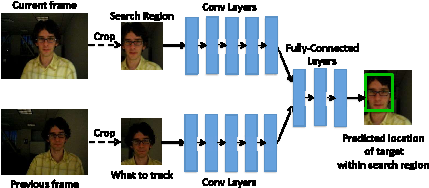
\includegraphics[width=0.8\linewidth]{figures/theoretical_foundations/goturn_framework.pdf}}
    \caption[\Gls{goturn} architecture]{The architecture of \gls{goturn} showing the input as a search region from the current frame where the target from the previous frame is to be searched for. The network essentially learns to localize the target within the cropped region. \externalsrc{\cite{held2016goturn}}}
    \label{fig:GOTURNFramework}
\end{figure}

\subsection{Fully Convolutional Tracking}
\label{ssec:FullyConvolutionalTracking}

We will start with a discussion about approaches that are so-called \emph{fully convolutional}. Transfer learning, e.g., exploiting an already pre-trained \gls{cnn} model to extract visual features, often comes with one drawback: the model accepts only a fixed input size. Although newer architectures can handle variable input size, this trait is more prevalent in object detection and segmentation than in basic task of image classification. A common approach is to resize the image to the required dimension, but this may significantly distort important features. Using fully connected layers demands known dimensions in advance, which is complicated to acquire when dealing with input of diverse shape. Convolutional layers are invariant to input size, therefore an avoidance of fully connected layers may provide an answer. An efficient solution to replace fully connected layers utilizes $1 \times 1$ convolutions notably propagated in \modelname{Network In Network} model~\cite{lin2014netinnet}. $1 \times 1$ filters were also used in the \modelname{Inception} architecture for dimensionality reduction and at the same time to increase the dimensionality of feature maps~\cite{szegedy2015resnet}.

The \glspl{cnn} provide valuable spatial clues about the image content. As we touched upon in section~\ref{ssec:ConvolutionalNeuralNetworks}, convolutional layers placed at the bottom (beginning) of the model tend to capture elementary details useful for discriminating between targets of similar appearance, whilst top layers (at the end) seize more abstract information regarding separate object categories. Thus, interclass variations are thoroughly captured in the top layers, and intraclass variations conversely in the bottom layers (Fig.~\ref{fig:FullyCNNTrackingFeatureMaps}). This concept led the authors of~\cite{wang2015votcnn} to propose a fully convolutional visual object tracker that exploits different layers of the pre-trained VGG network~\cite{simonyan2015verydeepcnn} (Fig.~\ref{fig:FullyCNNTrackingSNetGNet}). Thus, the model responsible for extracting visual features is no longer treated as a black-box. An in-depth study was conducted on the properties of \gls{cnn} features of the offline pre-trained model for the task of classification of ImageNet dataset~\cite{deng2009imagenet}. It was found out, as suggested above, that characterization from different perspectives is provided by convolutional layers at different levels. Moreover, only a small subset of neurons is actually relevant for the tracking process itself. In connection with this, a feature map selection method was developed to aid in the removal of irrelevant (noisy) feature maps, with a consequence of reducing computational complexity while improving tracking accuracy.

The motivation for the utilization of different convolutional layers was that existing appearance-based tracking methods adopted either generative or discriminative models for separating the foreground from the background~\cite{wang2015votcnn}. To denote the distinction between the two, assume a classification task with the goal of estimating a function $f: X \to Y$, or $\probgiven{Y}{X}$, where $X$ represents the data and $Y$ the associated labels. A generative classifier would estimate parameters $\probgiven{X}{Y}$ and $\prob{Y}$ (in essence, the joint probability $\prob{X, Y}$) from the training data and then use the Bayes' rule to compute $\probgiven{Y}{X}$. On the other hand, a discriminative classifier would estimate parameters of $\probgiven{Y}{X}$ from the training data directly~\cite{ng2002discriminative}. The reliance of such foreground-background separation models on low-level hand-crafted features is considered a major drawback thanks to the incapability to capture semantic information and not being robust to appearance changes. The use features generated by \glspl{cnn} resolved much of such issues.

\begin{figure}[t]
    \centering
    \begin{subfigure}[b]{0.13\textwidth}
        \centering
        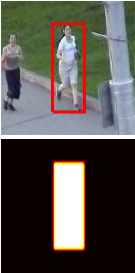
\includegraphics[width=\textwidth]{figures/theoretical_foundations/fully_cnn_tracking_feature_maps_1.pdf}
        \caption[]{}
    \end{subfigure}
    \hfill
    \begin{subfigure}[b]{0.39\textwidth}
        \centering
        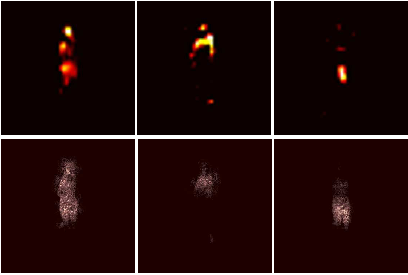
\includegraphics[width=\textwidth]{figures/theoretical_foundations/fully_cnn_tracking_feature_maps_2.pdf}
        \caption[]{}
    \end{subfigure}
    \hfill
    \begin{subfigure}[b]{0.39\textwidth}
        \centering
        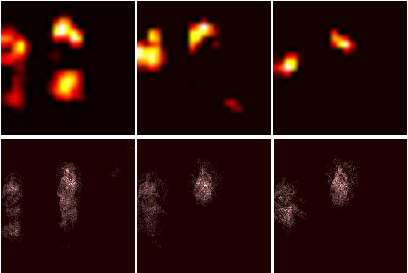
\includegraphics[width=\textwidth]{figures/theoretical_foundations/fully_cnn_tracking_feature_maps_3.pdf}
        \caption[]{}
    \end{subfigure}
    \caption[Fully convolutional tracking]{A \gls{cnn} model trained on image classification task carries spatial information. (a) Input image with an associated ground truth mask. (b) Visualization of feature maps from convolutional layers placed at the bottom of the model, capturing differences between foreground and background of a particular object instance. (c) As opposed to the previous group of images, a more holistic, abstract view on the object category itself is provided by feature maps from top convolutional layers. The top row in the (b) and (c) represents feature maps, whereas the bottom row represents the corresponding saliency map with spatial information of the category. \externalsrc{\cite{wang2015votcnn}}}
    \label{fig:FullyCNNTrackingFeatureMaps}
\end{figure}

Authors of~\cite{wang2015votcnn} put together a list of three observations that summarize properties of the fully convolutional nature of a tracker proposed by them.
\begin{itemize}
    \item Despite a large receptive field of \gls{cnn} feature maps, few of them are activated and they are sparsely distributed, localized, and correlated to the regions of semantic objects.
    \item The majority of the feature maps can be considered noisy or irrelevant when discriminating a specific target object (foreground) from the background.
    \item Different layers encode different types of features (related to the intraclass or interclass variations discussed at the beginning).
\end{itemize}
The proposed architecture in accordance to the aforementioned observation is described in Fig.~\ref{fig:FullyCNNTrackingFeatureMaps} and Fig.~\ref{fig:FullyCNNTrackingSNetGNet}.

\begin{figure}[t]
    \centerline{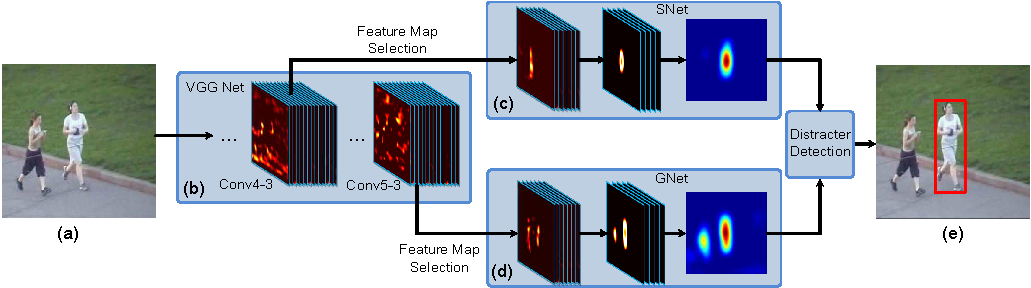
\includegraphics[width=\linewidth]{figures/theoretical_foundations/fully_cnn_tracking_snet_gnet.pdf}}
    \caption[Architecture of fully convolutional tracking]{For a given image, a feature map selection is performed on two different layers of the VGG network~\cite{simonyan2015verydeepcnn} to select the most relevant ones. This selection is handled as a heat map regression problem. A general network (GNet) captures the category information, whilst the specific network (SNet) captures visual traits based on which the foreground is separated from the background. Two heat maps are produced by these networks forming a basis for subsequent target localization. Both of these networks have to be initialized in the first frame. Afterward, when a new frame is to be processed, a region of interest is centered at the last target location, and the whole process repeats. \externalsrc{\cite{wang2015votcnn}}}
    \label{fig:FullyCNNTrackingSNetGNet}
\end{figure}

\subsection{Tracking Using Siamese Networks}
\label{ssec:TrackingUsingSiameseNetworks}

Even though \glspl{cnn} condense valuable visual information into low dimensional space upon which a tracker may be built, it is still not sufficient in many situations during object tracking. The object representation from convolutional layers trained on image classification is not robust enough for dramatic visual changes and occlusion of varying intensity. As we discussed in section~\ref{sec:LatentSpacesAndEmbeddings} dedicated to metric spaces and embeddings, an object representation supporting re-identification requires different types of models, one of which is a \emph{Siamese network} (section~\ref{ssec:SiameseAndTripletNetworks}). We have already mentioned our intention of utilizing custom metric space for tracking, and~\cite{bertinetto2016siamfc} were among the first ones to successfully demonstrate it.

Authors of~\cite{bertinetto2016siamfc} approved of the idea that visual feature extraction using \glspl{cnn} is pertinent to the robustness of the tracking algorithm, yet they advocated to train the visual model to a more general task of similarity learning rather than just classification. This observation and its further implementation was the main contribution of their work, achieving \gls{sota} performance back then. Broadly speaking, they trained a \emph{fully convolutional} Siamese network to locate an \emph{exemplar} image within a larger \emph{search} image (Fig.~\ref{fig:FullyCNNSiamTrackingArch}). The model got the name \modelname{Siam-FC}. We mentioned this to make the comparison easier because a lot of follow-up work has been done, producing models such as \modelname{SA-Siam}~\cite{he2018twofoldsiam}, \modelname{Siam-RPN}~\cite{li2018siamrpn}, \modelname{Siam-Mask}~\cite{wang2019siammask}, \modelname{Siam-Mask-E}~\cite{chen2019rotbboxes} and so forth.

Let $\gamma$ be a transformation that extracts visual features from the input, and $g$ be the function that combines two representations produced by the function $\gamma$. Siamese networks apply this identical transformation $\gamma$ to both inputs, search image $x$ and exemplar image $z$, and then combine the result as $\func{f}{x, z} = \func{g}{\func{\gamma}{x}, \func{\gamma}{z}}$. As such, when trivial distance or similarity measure is computed by the function $g$, then $\gamma$ can be deemed as the already introduced embedding.

\begin{figure}[t]
    \centerline{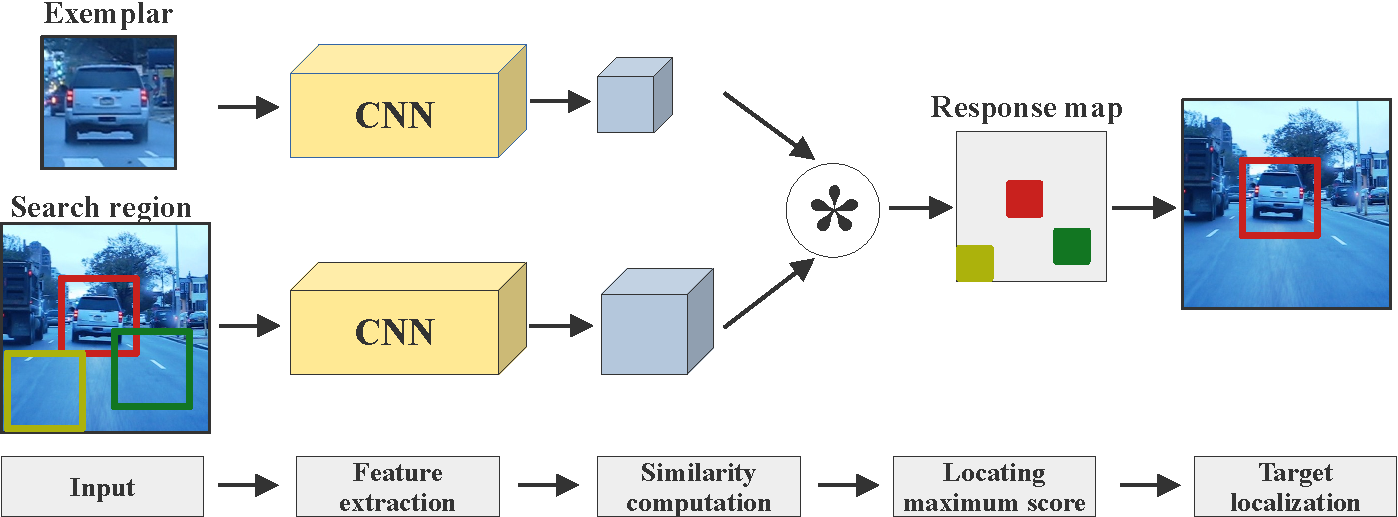
\includegraphics[width=0.7\linewidth]{figures/theoretical_foundations/fully_cnn_siam_tracking_architecture.pdf}}
    \caption[\modelname{Siam-FC} architecture]{The fully-convolutional Siamese architecture produces a scalar-valued score map, the size of which depends on the size of the search image. The similarity function is computed for all sub-windows within the search image and stored in a 2D score map, rather than just a pure 1D embedding vector. This computation requires only one evaluation. In this image, the red and blue pixels in the output score map represent similarity values for the two sub-windows on the input. Best viewed in color. \externalsrc{\cite{bertinetto2016siamfc}}}
    \label{fig:FullyCNNSiamTrackingArch}
\end{figure}

The use of the Siamese architecture spawned a lot of follow-up work, and we will describe some that serve our purposes. A team of authors in~\cite{he2018twofoldsiam} made the following observation: features learned in an image classification task (denoted as semantic features) complement features learned in a similarity matching task (denoted as appearance features). They also suitably commented that the key to designing a high-performance tracker is to harness expressive features that are simultaneously discriminative and generalized. In light of this, they developed a model consisting of a semantic and an appearance branch (see Fig.~\ref{fig:TwofoldSiameseNetArchitecture}), with each branch being represented by a standard similarity-learning Siamese network (as in \modelname{Siam-FC}~\cite{bertinetto2016siamfc}). However, an important distinction is that these two branches were trained separately, making them effectively heterogeneous to avoid any sharing of information. They reported that both branches were less powerful when trained jointly than when trained separately. The rationale behind such a decision was that each branch provides different features produced at different levels of abstraction, yet they complement each other. The merge of their respective outputs happens only during the testing time.

\begin{figure}[t]
    \centerline{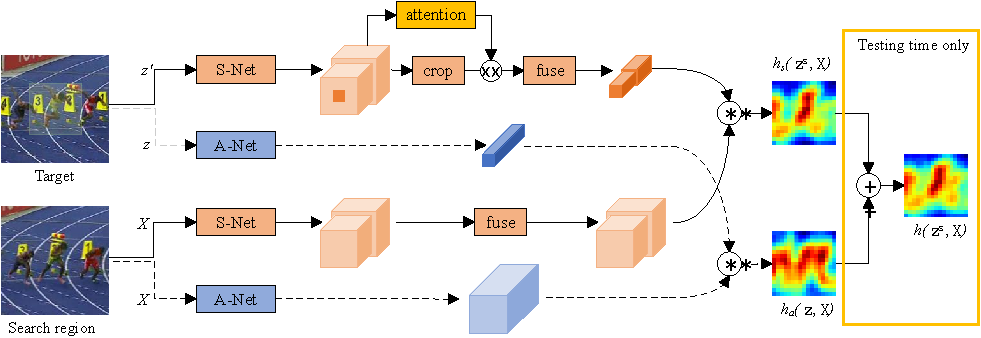
\includegraphics[width=\linewidth]{figures/theoretical_foundations/twofold_siamese_net_architecture.pdf}}
    \caption[\modelname{SA-Siam} architecture]{The architecture of the \modelname{SA-Siam} network. The \modelname{A-Net} represents the appearance network and the \modelname{S-Net} represents the semantic network. For the reason that this work builds on \modelname{Siam-FC} model~\cite{bertinetto2016siamfc}, structures connected by dotted lines are exactly the same as in the \modelname{Siam-FC} model. The last two convolutional layers provide features that are extracted afterward. The attention model determines the weight of each feature channel by simultaneous consideration of target and context information. The fusion module is trivial and uses just $1 \times 1$ convolutions. As shown on the right, combining branches is allowed only when testing. \externalsrc{\cite{he2018twofoldsiam}}}
    \label{fig:TwofoldSiameseNetArchitecture}
\end{figure}

The \modelname{SA-Siam} receives an input as a pair of image patches (Fig.~\ref{fig:TwofoldSiameseNetArchitecture}) cropped from the initial (target) frame and the current frame. Let $z$, $z^s$ and $X$ be the image of target, target including the surrounding context and the search region, respectively. Dimensions of $x^s$ and $X$ are identical, $W_s \times H_s \times 3$. Dimensions of the target $z$ located in the exact center of the region of $z^s$ are $W_t \times H_t \times 3$, such that $W_t < W_s$ and $H_t < H_s$. The appearance branch (\modelname{A-Net}) takes $\rbrackets{z, X}$ as input and essentially clones the entire \modelname{Siam-FC} network. Let $\func{f_a}{\cdot}$ denote the visual features extracted by the \modelname{A-Net}. Then, the response map of this branch is given by
\begin{equation}
    \func{h_a}{z, X} = \func{corr}{\func{f_a}{z}, \func{f_a}{X}},
\end{equation}
where $\func{corr}{\cdot}$ is the correlation operation. The training of this branch is rather straightforward thanks to the abundance of training pairs $\rbrackets{z_i, X_i}$ with their related response map $Y_i$, for $i = 1, \dots, N$, with $N$ being the no. of chosen training samples. The parameters $\theta_a$ of the \modelname{A-Net} model are optimized from scratch by minimizing the logistic loss function $\func{\mathcal{L}}{\cdot}$:
\begin{equation}
    \label{eq:ANetModelTraining}
    \underset{\theta_a}{\argmin}
    \frac{1}{N}
    \cbrackets{
        \func{\mathcal{L}}{
            \func{h_a}{z_i, X_i; \theta_a},
            Y_i
        }
    }.
\end{equation}

Analogically, the semantic branch (\modelname{S-Net}) assumes as input a pair $\rbrackets{z^s, X}$. Contrary to the \modelname{A-Net}, this model is pre-trained for the image classification task and its weights are frozen during the training phase. These last two convolutional layers of this model are of primary interest as their features provide abstraction at distinct levels. However, spatial resolutions are not alike. Let $\func{f_s}{\cdot}$ be the concatenated multilevel features. For the correlation operation ($\func{corr}{\cdot}$) to be usable, a special fusion module is introduced, implemented by a simple $1 \times 1$ convolution layer. The fusion operation is applied to features within the same layer, and this fused feature vector will be referred to as $\func{g}{\func{f_s}{X}}$.

Semantic features of higher-level are robust to appearance variation. This contributes to the generalization ability of the tracker but exacerbates its discriminative abilities. To circumvent this, the attention module is presented. The reasoning is that individual feature channels have varying importance for object tracking as far as different targets are concerned. The goal is then to assign a degree of importance (weight) to each channel for each target. Still, the target information is not sufficient, so the context must be supplied, too. The proposed attention module thus processes the feature map of $z^s$ instead of just $z$. Although the use of multilevel features in conjunction with the attention module delivers substantial progress for the semantic branch, it would be counterproductive for the appearance branch. Appearance features extracted from different convolutional layers lack sufficient differences in terms of expressiveness, as these features are dense whereas high-level semantic features are very sparse.

The attention module operates channel-wise. Assume the $i^{\text{th}}$ channel from some convolutional feature map with spatial dimensions of $22 \times 22$ is being processed. The tracking target is contained in the center, covering a region of $6 \times 6$. The entire feature map is divided into a grid of $3 \times 3$ cells. Within each grid, a max-pooling operation is applied followed by a simple neural network consisting of just $1$ hidden layer. The weight coefficient $\zeta_i$ for the particular $i^{\text{th}}$ channel is generated by the sigmoid activation function (Fig.~\ref{fig:TwofoldSiameseNetAttentionModule}). The attention module incurs negligible computational overhead as it's only active during the target processing on the first frame. Later on, the weight coefficient is used to scale each feature map according to its importance. The response map for the semantic branch is produced as
\begin{equation}
    \func{h_s}{z^s, X} =
    \func{corr}{
        \func{g}{\zeta \cdot \func{f_s}{z}},
        \func{g}{\func{f_s}{X}}
    },
\end{equation}
where the no. of elements of $\zeta$ is equal to the no. of channels in $\func{f_s}{z}$, and the operator $\cdot$ indicates an element-wise multiplication.

\begin{figure}[t]
    \centerline{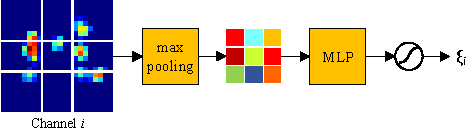
\includegraphics[width=0.6\linewidth]{figures/theoretical_foundations/twofold_siamese_net_attention_module.pdf}}
    \caption[\modelname{S-Net} attention module]{The attention module of the \modelname{S-Net} network. \externalsrc{\cite{he2018twofoldsiam}}}
    \label{fig:TwofoldSiameseNetAttentionModule}
\end{figure}

When training the \modelname{S-Net} branch, only the fusion and the attention modules are updated. No fine-tuning techniques are taken advantage of, regardless of the potential improvement of the semantic branch alone. Authors informed about such experiments, and they resulted in diminished overall performance thanks to \modelname{A-Net} and \modelname{S-Net} becoming less heterogeneous. Let $\rbrackets{\subsup{z}{i}{s}, X_i}$ with their corresponding ground-truth response map $Y_i$, for $i = 1, \dots, N$, be the $N$ chosen training samples. The parameters $\theta_s$ of the \modelname{S-Net} model are fitted using the logistic loss function $\func{\mathcal{L}}{\cdot}$ (equal to equation~\ref{eq:ANetModelTraining})
\begin{equation}
    \label{eq:SNetModelTraining}
    \underset{\theta_s}{\argmin}
    \frac{1}{N}
    \cbrackets{
        \func{\mathcal{L}}{
            \func{h_a}{\subsup{z}{i}{s}, X_i; \theta_a},
            Y_i
        }
    }.
\end{equation}
The inference phase involves computation of the overall heat map for which a weighted average of the two produced heat maps is used as shown below:
\begin{equation}
    \func{h}{z, z^s, X} = \lambda \func{h_a}{z, X} + \rbrackets{1 - \lambda} \func{h_s}{z^s, X}.
\end{equation}
This introduces another hyperparameter $\lambda$ (where $0 < \lambda < 1$) that can in practice be reliably estimated from the validation dataset.

The series of Siamese-based architectures for tracking continued with the idea of using the \gls{rpn}~\cite{li2018siamrpn} (see section~\ref{ssec:FasterRCNN} for the same concept applied in object detection). Under the flag of end-to-end training, the \modelname{SiamRPN} model consists of a Siamese subnetwork for feature extraction (again, a duplicate of the \modelname{SiamFC}~\cite{bertinetto2016siamfc}) and \gls{rpn} as another subnetwork encompassing both classification and regression branch (Fig.~\ref{fig:SiamRPNNetArchitecture}). The notable contribution is that the proposed framework is formulated as a local one-shot detection task in the inference phase (the first work to make such a step) (Fig.~\ref{fig:SiamRPNOneShotDetection}). The template branch encodes the object appearance information for further foreground/background discrimination. Analogically, the \gls{bbox} from the first frame is the only exemplar for one-shot detection in the inference phase.

The region proposal subnetwork contains a pair-wise correlation section as well as a supervision section. Let $k$ denote the number of anchors. Then, the model has to output $2k$ channels for the classification and $4k$ channels for the regression. Following the established notation, the Siamese subnetwork produces feature maps $\func{\gamma}{z}$ and $\func{\gamma}{x}$. The pair-wise correlation splits $\func{\gamma}{z}$ into $\sbrackets{\func{\gamma}{z}}_{cls}$ and $\sbrackets{\func{\gamma}{z}}_{reg}$ while increasing the no. of channels (Fig.~\ref{fig:SiamRPNNetArchitecture}). Conversely, $\func{\gamma}{x}$ is also split into $\sbrackets{\func{\gamma}{x}}_{cls}$ and $\sbrackets{\func{\gamma}{x}}_{reg}$, but the no. of channels remains unchanged. The correlation, when computed on both branches, is given by
\begin{equation}
    \begin{aligned}
        \subsup{A}{w \times h \times 2k}{cls} &=
        \sbrackets{\func{\gamma}{x}}_{cls} \star \sbrackets{\func{\gamma}{z}}_{cls},\\
        \subsup{A}{w \times h \times 4k}{reg} &=
        \sbrackets{\func{\gamma}{x}}_{reg} \star \sbrackets{\func{\gamma}{z}}_{reg},
    \end{aligned}
\end{equation}
where the template feature maps $\sbrackets{\func{\gamma}{z}}_{cls}$ and $\sbrackets{\func{\gamma}{z}}_{reg}$ stand in place of kernels in the convolution operation signified by the $\star$ character.

\begin{figure}[t]
    \centerline{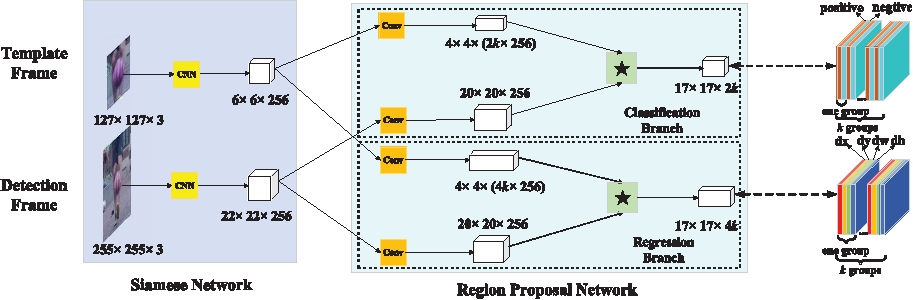
\includegraphics[width=\linewidth]{figures/theoretical_foundations/siam_rpn_architecture.pdf}}
    \caption[\modelname{Siam-RPN} architecture]{The pipeline starts with the original \modelname{Siam-FC} network followed by the \gls{rpn} which has two branches: classification and regression. The output of the two branches is obtained using a pair-wise correlation. Foreground/background classification and the box regression are given by the $17 \times 17 \times 2k$ and $17 \times 17 \times 4k$ feature maps, respectively. \externalsrc{\cite{li2018siamrpn}}}
    \label{fig:SiamRPNNetArchitecture}
\end{figure}

The noteworthy formulation of tracking as one-shot detection was proposed as follows. In general terms, the goal is to minimize the average loss $\mathcal{L}$ of a predictor function $\func{\psi}{x; W}$ by finding its parameters $W$. When computed over a dataset of $N$ samples $x_i$ with corresponding labels $y_i$, $\forall i = 1, \dots, N$, it is given by
\begin{equation}
    \label{eq:SiamRPNOneShotGeneral}
    \underset{W}{\argmin}
    \cbrackets{
        \frac{1}{N}
        \sum_{i = 1}^{N}
        \func{\mathcal{L}}{
            \func{\psi}{x_i; W},
            y_i
        }
    }.
\end{equation}
\emph{One-shot learning} aims to learn $W$ when only a single template $z$ is available.
Discriminative one-shot learning tackles a major challenge of \emph{learning to learn}, by finding a mechanism to integrate category information into the learner~\cite{bertinetto2016oneshot}. If we consider a meta-learning feed-forward function $\omega$ that maps $\rbrackets{z_i; W'}$ to $W$, then the problem can be stated as
\begin{equation}
    \label{eq:SiamRPNOneShotMetaLearning}
    \underset{W'}{\argmin}
    \cbrackets{
        \frac{1}{N}
        \sum_{i = 1}^{N}
        \func{\mathcal{L}}{
            \func{\psi}{x_i; \func{\omega}{z_i, W'}},
            y_i
        }
    }.
\end{equation}
In this setting, this objective function can be re-written in terms of the Siamese subnetwork feature extraction $\gamma$ and region proposal subnetwork $\Psi$ as
\begin{equation}
    \label{eq:SiamRPNOneShoCombo}
    \underset{W}{\argmin}
    \cbrackets{
        \frac{1}{N}
        \sum_{i = 1}^{N}
        \func{\mathcal{L}}{
            \func{\Psi}{\func{\gamma}{x_i; W}; \func{\gamma}{z_i; W}},
            y_i
        }
    }.
\end{equation}
The template branch provides training parameters to predict the kernel for the detection task, a typical example of the \emph{learning to learn} process. The template branch, therefore, embeds necessary category information into the kernel that is subsequently utilized for detection (Fig.~\ref{fig:SiamRPNOneShotDetection}). The last thing to consider is how to propose and then select the regions. One strategy is to discard boxes too far away from the object's center. A possible implementation is to keep $g \times g$ subregion of the $\subsup{A}{w \times h \times 2k}{cls}$ feature map resulting in $g \times g \times k$ anchors instead of $w \times h \times k$. This idea is the beginning of a further refined notion in future papers of the so-called \emph{centerness} that plays an important role in weighting \glspl{bbox}. Another strategy would be to use a cosine window to help in computing a penalty bound to a too large displacement in size and ratio. Afterwards, the \gls{nms} (section~\ref{ssec:NonMaximumSuppression}) is applied to get the final tracking \gls{bbox}.

\begin{figure}[t]
    \centerline{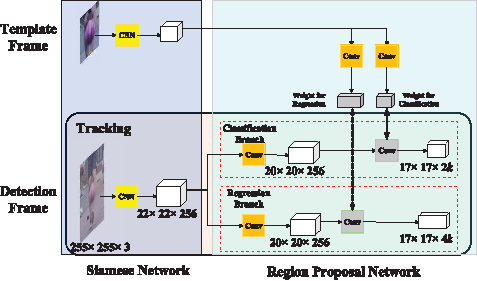
\includegraphics[width=0.7\linewidth]{figures/theoretical_foundations/siam_rpn_one_shot_detection.pdf}}
    \caption[Tracking as one-shot detection]{Tracking is framed as one-shot detection here. First, the template branch predicts the weights of the kernels for the \gls{rpn} using the first frame. Later on, only the detection branch is retained so the framework can be thought of as a local detection network. \externalsrc{\cite{li2018siamrpn}}}
    \label{fig:SiamRPNOneShotDetection}
\end{figure}

Later on, a fork of publications emerged with an endeavor to improve the tracking performance by estimating not only a regular axis-aligned \gls{bbox}, but a rotated box, too. Put into perspective, the rotated \gls{bbox}, as opposed to an ordinary, axis-aligned, contains the minimal amount of background pixels~\cite{chen2019rotbboxes}. Thus, datasets with rotated \glspl{bbox} provide tighter enclosed boxes. Additionally, the orientation information may be useful for solving different computer vision problems, such as action classification.

Inspiration from techniques for the problem of object segmentation yielded another approach where the tracking process was assisted with additional semi-supervised object segmentation~\cite{wang2019siammask}. The relevant contribution is the augmentation of the training loss with a binary segmentation task. Further, once trained, the model (dubbed \modelname{Siam-MASK}) relies exclusively upon a single \gls{bbox} initialization and operates online while producing rotated \glspl{bbox} instead of axis-aligned ones together with class-agnostic object segmentation masks. Notwithstanding its convenience, a single rectangle frequently fails to represent the object appropriately, hence the motivation to generate additional segmentation masks.

As always, the \modelname{SiamFC}~\cite{bertinetto2016siamfc} was employed as the fundamental building block. However, a notable alternation consisted of the use of a depth-wise cross-correlation layer instead of a simple cross-correlation layer. The latter one compresses all the information into one channel, impeding the potential to encode richer information about the target object. As a reminder, the original model used $6 \times 6 \times 128$ and $22 \times 22 \times 128$ tensors to produce a $17 \times 17 \times 1$ response map (Fig.~\ref{fig:FullyCNNSiamTrackingArch}). Here, a multi-channel response maps are utilized (Fig.~\ref{fig:SiamMaskArchitecture}).

\begin{figure}[t]
    \centering
    \begin{subfigure}[b]{0.68\textwidth}
        \centering
        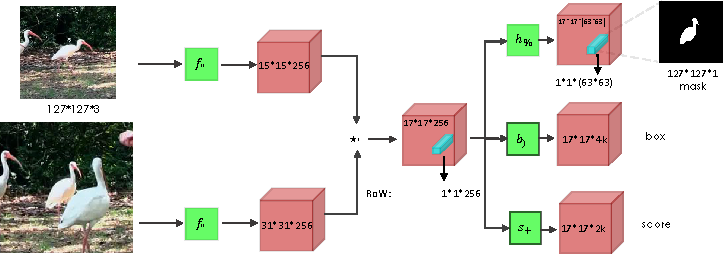
\includegraphics[width=\textwidth]{figures/theoretical_foundations/siam_mask_architecture_3_branch.pdf}
        \caption[]{}
    \end{subfigure}
    \hfill
    \begin{subfigure}[b]{0.31\textwidth}
        \centering
        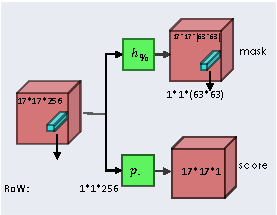
\includegraphics[width=\textwidth]{figures/theoretical_foundations/siam_mask_architecture_2_branch_head.pdf}
        \caption[]{}
    \end{subfigure}
    \caption[\modelname{Siam-Mask} architecture]{A schematic illustration of the two \modelname{Siam-Mask} variants: (a) a three-branch architecture (full), (b) a two-branch architecture (head). Depth-wise correlation layers are adopted again. \externalsrc{\cite{wang2019siammask}}}
    \label{fig:SiamMaskArchitecture}
\end{figure}

Let $z$ and $x$ be the exemplar and the search image, respectively. Then, these two inputs are processed by the same \gls{cnn} $f_\theta$ to yield $g_\theta$ using the cross-correlation as follows:
\begin{equation}
    \label{eq:SiamMaskCrossCorrelation}
    \func{g_\theta}{z, x} = \func{f_\theta}{z} \star \func{f_\theta}{x}.
\end{equation}
Authors contrived the term \gls{row} to represent each spatial element of the response map given by the left hand side of equation~\ref{eq:SiamMaskCrossCorrelation}. In that regard, the similarity between the exemplar $z$ and the $n$-th candidate window in $x$ is declared as $\func{\subsup{g}{\theta}{n}}{z, x}$. Throughout the training phase, $w \times h$ binary masks (one for each \gls{row}) using a trivial two-layer neural network $h_\phi$ are predicted. Let $\mtx{M_n}$ be the predicted segmentation mask corresponding to the $n$-th \gls{row},
\begin{equation}
    \mtx{M_n} = \func{h_\phi}{\func{\subsup{g}{\theta}{n}}{z, x}}.
\end{equation}
A ground-truth binary label $y_n \in \cbrackets{\pm 1}$ is assigned to each \gls{row} as well as pixel-wise ground-trith mask $\mtx{C_n}$ with dimensions $w \times h$. Let $\mtx{C}_n^{i,j} \in \cbrackets{\pm 1}$ denote the label corresponding to pixel at position $\rbrackets{i, j}$ within the segmentation mask in the $n$-th \gls{row}. The mask prediction task is driven by the binary logistic regression loss function $\mathcal{L}_{mask}$ over all \glspl{row}:
\begin{equation}
    \func{\mathcal{L}_{mask}}{\theta, \phi} =
    \sum_n
    \rbrackets{
        \frac{1 + y_n}{2wh}
        \sum_{i}
        \sum_{j}
        \func{\log}{1 + e^{-\mtx{C}_n^{i,j} \mtx{M}_n^{i,j}}}
    }.
\end{equation}

An incremental improvement of \modelname{Siam-Mask} model came when~\cite{chen2019rotbboxes} proposed a novel, efficient algorithm for the estimation of the \gls{bbox} rotation when the object segmentation mask is given. Particularly, a mask produced by the \modelname{Siam-Mask} model, as this work builds on top of~\cite{wang2019siammask}, under the derived name \modelname{Siam-Mask-E}. In addition, their approach can be used to generate a rotated box ground truth from any segmentation datasets to train a rotation angle regression model.

To estimate the rotation angle, they adopted the least-squared scheme as part of the ellipse fitting algorithm. Considering the standard conic equation
\begin{equation}
    ax^2 + bxy + cy^2 + dx + ey + f = 0,
\end{equation}
the ellipse can be formulated by adding a constraint
\begin{equation}
    b^2 - 4ac < 0,
\end{equation}
where $a$, $b$, $c$, $d$, $e$, and $f$ are the coefficients of the ellipse and $x$, $y$ represent any point on the ellipse. Let $\vectt{a}{a, b, c, d, e, f}$ and $\vectt{x}{x^2, xy, y^2, x, y, 1}$. The ellipse equation can then be written as
\begin{equation}
    \func{F}{\vect{x}} = \vect{x}^T\vect{a} = 0.
\end{equation}
Assume a dataset of $N$ points, $\mset{A} = \cbrackets{\rbrackets{x_1, y_1}, \rbrackets{x_2, y_2}, \dots, \rbrackets{x_N, y_N}}$, and a task of fitting an ellipse to the dataset $\mset{A}$. The goal is to find the coefficients of the vector $\vect{a}$, as determined by the objective function
\begin{equation}
    \underset{\vect{a}}{\argmin} \sum_{i = 1}^{N} {\func{F}{\vect{x}_i}}^2,
\end{equation}

\begin{figure}[t]
    \centerline{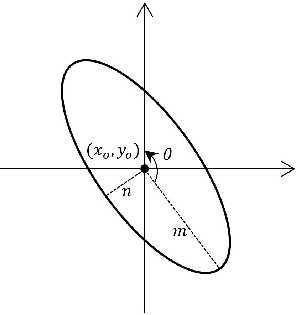
\includegraphics[width=0.4\linewidth]{figures/theoretical_foundations/fast_vot_rot_bbox_ellipse.pdf}}
    \caption[Ellipse notation]{Ellipse notation: $\rbrackets{x_0, y_0}$ is the center point around which the ellipse with semi-major axis $m$ and semi-minor axis $n$ is rotated by the angle $\theta$ in counter-clockwise direction. \externalsrc{\cite{chen2019rotbboxes}}}
    \label{fig:FastVOTRotBBOXEllipse}
\end{figure}
where $\vect{x}^T = \sbrackets{\subsup{x}{i}{2}, x_i y_i, \subsup{y}{i}{2}, x_i, y_i, 1}$ and $\mset{A}_i = \rbrackets{x_i, y_i}$.

For the upcoming description, we advise to follow the description for Fig.~\ref{fig:FastVOTRotBBOXFitting}. Once the coefficients are estimated, the rotation angle $\theta$ around the center point $\rbrackets{x_0, y_0}$ with semi-major $m$ and semi-minor axis $n$ are trivial to obtain (Fig.~\ref{fig:FastVOTRotBBOXEllipse}). The 2D affine transformation matrix
\begin{equation}
    \mtx{T} =
    \begin{bmatrix}
        \func{\cos}{\theta} &
        \func{\sin}{\theta} &
        \rbrackets{1 - \func{\cos}{\theta}}x_0 - \func{\sin}{\theta} y_0\\
        -\func{sin}{\theta} &
        \func{\cos}{\theta} &
        \func{\sin}{\theta} x_0 - \rbrackets{1 - \func{\cos}{\theta}} y_0
    \end{bmatrix}
\end{equation}
is thereafter used to produce the set $\mset{M'}$, which contains the transformed (rotated and translated) points belonging to the input segmentation mask, denoted by the set $\mset{M}$, as
\begin{equation}
    \mset{M'} =
    \cbrackets{
        \mtx{T}
        \sbrackets{x, y, 1}^T
        \ | \
        \forall \rbrackets{x, y} \in \mset{M}
    }.
\end{equation}
Computing the \gls{bbox} $\vect{G}$ into which the ellipse after being transformed by $\mtx{T}$ is inscribed is rather straightforward:
\begin{equation}
    \vectt{G}{x_0 - n, y_0 - m, x_0 + n, y_0 + m}.
\end{equation}
Considering the extreme values for coordinates $x$ and $y$ below:
\begin{equation}
    \begin{aligned}
        &x_{min} = \min \cbrackets{x\ |\ \forall x \in \mset{M'}},
        \quad
        &x_{max} = \max \cbrackets{x\ |\ \forall x \in \mset{M'}},\\
        &y_{min} = \min \cbrackets{y\ |\ \forall y \in \mset{M'}},
        \quad
        &y_{max} = \max \cbrackets{y\ |\ \forall y \in \mset{M'}},
    \end{aligned}
\end{equation}
then the the min-max axis-aligned \gls{bbox} $\vect{B}$ is given by
\begin{equation}
    \vectt{B}{x_{min}, y_{min}, x_{max}, y_{max}}.
\end{equation}
Combining $\vect{G}$ and $\vect{B}$ we have the intersection \gls{bbox} $\vect{R}$ calculated using the following equation:
\begin{equation}
    \vectt{R}{
        \max \cbrackets{\vect{G_1}, \vect{B_1}},
        \max \cbrackets{\vect{G_2}, \vect{B_2}},
        \min \cbrackets{\vect{G_3}, \vect{B_3}},
        \min \cbrackets{\vect{G_4}, \vect{B_4}}
    }.
\end{equation}
Let $\mset{R}$ be the set containing vertices of the box $\vect{R}$, thus
\begin{equation}
    \mset{R} = \cbrackets{
        \rbrackets{\vect{R_1}, \vect{R_2}},
        \rbrackets{\vect{R_3}, \vect{R_2}},
        \rbrackets{\vect{R_3}, \vect{R_4}},
        \rbrackets{\vect{R_1}, \vect{R_4}}
    }.
\end{equation}
The last step, the conversion of the transformed coordinates back to the original image coordinates, is performed using the inverse affine transformation matrix $\mtx{T}^{-1}$. The result of this operation is accomplished by
\begin{equation}
    \mset{R'} =
    \cbrackets{
        \mtx{T}^{-1}
        \sbrackets{x, y, 1}^T
        \ | \
        \forall \rbrackets{x, y} \in \mset{R}
    }.
\end{equation}

\begin{figure}[t]
    \centering
    \begin{subfigure}[b]{0.135\textwidth}
        \centering
        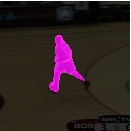
\includegraphics[width=\textwidth]{figures/theoretical_foundations/fast_vot_rot_bbox_algo_01.pdf}
        \caption[]{}
    \end{subfigure}
    \hfill
    \begin{subfigure}[b]{0.135\textwidth}
        \centering
        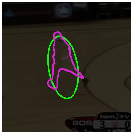
\includegraphics[width=\textwidth]{figures/theoretical_foundations/fast_vot_rot_bbox_algo_02.pdf}
        \caption[]{}
    \end{subfigure}
    \hfill
    \begin{subfigure}[b]{0.135\textwidth}
        \centering
        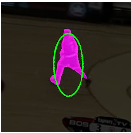
\includegraphics[width=\textwidth]{figures/theoretical_foundations/fast_vot_rot_bbox_algo_03.pdf}
        \caption[]{}
    \end{subfigure}
    \hfill
    \begin{subfigure}[b]{0.135\textwidth}
        \centering
        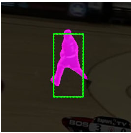
\includegraphics[width=\textwidth]{figures/theoretical_foundations/fast_vot_rot_bbox_algo_04.pdf}
        \caption[]{}
    \end{subfigure}
    \hfill
    \begin{subfigure}[b]{0.135\textwidth}
        \centering
        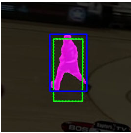
\includegraphics[width=\textwidth]{figures/theoretical_foundations/fast_vot_rot_bbox_algo_05.pdf}
        \caption[]{}
    \end{subfigure}
    \hfill
    \begin{subfigure}[b]{0.135\textwidth}
        \centering
        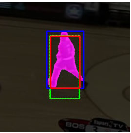
\includegraphics[width=\textwidth]{figures/theoretical_foundations/fast_vot_rot_bbox_algo_06.pdf}
        \caption[]{}
    \end{subfigure}
    \hfill
    \begin{subfigure}[b]{0.135\textwidth}
        \centering
        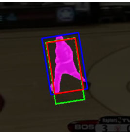
\includegraphics[width=\textwidth]{figures/theoretical_foundations/fast_vot_rot_bbox_algo_07.pdf}
        \caption[]{}
    \end{subfigure}
    \caption[Rotated \gls{bbox} by ellipse fitting]{(a) Edge pixels of the input segmentation mask, (b) ellipse fitting, (c) the affine transformation is computed and the points belonging to the mask are rotated and translated, (d) the ellipse is then inscribed into a rectangular box, (e) this box is then intersected with the min-max rectangular box, (f) the intersection box, (g) inverse affine transformation. \externalsrc{\cite{chen2019rotbboxes}}}
    \label{fig:FastVOTRotBBOXFitting}
\end{figure}

The idea to employ fully convolutional networks seems to pertain to the modern computer vision community. Besides a simpler model, the fully convolutional design often leads to a reduced number of hyperparameters. One such an architecture (a descendant of the famous \modelname{Siam-FC}~\cite{bertinetto2016siamfc} model) has been recently proposed, named \modelname{Siam-CAR}~\cite{guo2019siamcar}. This approach relies on the decomposition of the task of \gls{vot} into two subproblems: classification for pixel category and regression for object \gls{bbox} at the given pixel. The leading concept of the article is that this tracker operates in an end-to-end, per-pixel manner. The authors managed to avoid the use of anchors as well as region proposals, hence reducing the need for human intervention. The use of the two aforementioned traits commonly leads to sensitivity to dimensions and aspect ratios of the anchor boxes, which requires expertise on hyperparameter tuning for successful tracking.

\begin{figure}[t]
    \centerline{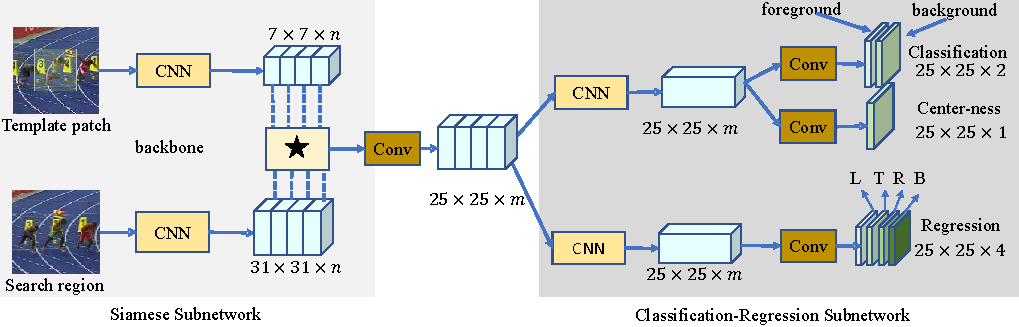
\includegraphics[width=\linewidth]{figures/theoretical_foundations/siamcar_architecture.pdf}}
    \caption[\modelname{Siam-CAR} architecture]{\modelname{Siam-CAR} architecture. The left side consists of the original \modelname{Siam-FC}~\cite{bertinetto2016siamfc} model, with a simple amendment of using depth-wise correlation for multi-channel response map extraction. The right side depicts the subnetworks for foreground/background classification and \gls{bbox} regression. \externalsrc{\cite{guo2019siamcar}}}
    \label{fig:SiamCARArchitecture}
\end{figure}

Let $R$ be the response map produced by a depth-wise correlation between the features extracted by the Siamese network from the exemplar $Z$ and the target $X$ (Fig.~\ref{fig:SiamCARArchitecture}). Then,
\begin{equation}
    R = \func{\gamma}{X} \star \func{\gamma}{Z}.
\end{equation}
An indispensable part of localization are low-level features like edges, corners, and so on, whereas high-level features strengthen the representational power from the semantic point of view, which is crucial for discrimination. Authors fused low-level and high-level features from the last $3$ residual blocks of the \modelname{ResNet-50} backbone (indicated by the $\func{F_3}{X}$, $\func{F_4}{X}$ and $\func{F_5}{X}$), forming a unity after concatenation (in case of $X$):
\begin{equation}
    \func{\gamma}{X} = \func{cat}{\func{F_3}{X}, \func{F_4}{X}, \func{F_5}{X}}.
\end{equation}
The resulting $\func{\gamma}{X}$ contains $3 \times 255$ channels since all $\func{F_i}{X}, \forall i = 3, 4, 5$, include $256$ channels. The response map $R$ is then convoluted with $1 \times 1$ kernel to reduce its dimension to $256$ channels, giving the reduced response map $R^*$.

At a later stage, the response map $\subsup{R}{w \times h \times m}{*}$ extracted by the Siamese subnetwork serves for classification and regression branches, producing feature maps $\subsup{A}{w \times h \times 2}{cls}$ and $\subsup{A}{w \times h \times 4}{reg}$, respectively. Each point $\rbrackets{i, j, :}$ in $\subsup{A}{w \times h \times 2}{cls}$ contains a $2D$ vector representing the foreground and background scores. Analogically, each point $\rbrackets{i, j, :}$ in $\subsup{A}{w \times h \times 4}{reg}$ contains a $4D$ vector $\vectt{t_{i, j}}{l, t, r, b}$ specifying distance from the corresponding location to the $4$ sides of the \gls{bbox} in the input search region. Let $\rbrackets{x_0, y_0}$ and $\rbrackets{x_1, y_1}$ denote the top-left and bottom-right corners of the ground-truth \gls{bbox} and $\rbrackets{x, y}$ the corresponding location of a point $\rbrackets{i, j}$. The regression target $\vect{\tilde{t}_{i, j}}$ at $\subsup{A}{w \times h \times 4}{reg} \rbrackets{i, j, :}$ can be computed as:
\begin{equation}
    \vectt{\tilde{t}_{i, j}}{x - x_0, y - y_0, x_1 - x, y_1 - y}.
\end{equation}
The regression loss is consequently computed using the \gls{iou} (section~\ref{sssec:IntersectionOverUnion}) algorithm,
\begin{equation}
    \label{eq:SiamCARRegLoss}
    \mathcal{L}_{reg} =
    \frac{1}{\sum \func{\mathbbm{1}}{\vect{\tilde{t}_{i, j}}}}
    \sum_{i, j}
    \func{\mathbbm{1}}{\vect{\tilde{t}_{i, j}}}
    \func{\mathcal{L}_{IOU}}{\func{A^{reg}}{i, j, :}, \vect{\tilde{t}_{i, j}}},
\end{equation}
which was proposed as part of loss function (given by $\func{\mathcal{L}_{IOU}}{\cdot}$) in~\cite{yu2016unitbox}. The indicator function $\func{\mathbbm{1}}{\cdot}$ evaluated to $1$ if the given location lies within a ground truth \gls{bbox}, otherwise the value is $0$. An important observation was made that locations further away from the object center may aggravate the predicted box as they can be considered of low-quality. To diminish the effect of such locations, another branch alongside the classification branch to suppress the outliers is introduced, based on the concept of \emph{centerness} (section~\ref{ssec:FullyConvolutioanlObjectDetection}, Fig.~\ref{fig:FCOSCenterness}) borrowed from the~\cite{tian2019fcos}. This branch outputs a feature map $\subsup{A}{w \times h \times 1}{cen}$, where each point indicates the \emph{centerness} score for the corresponding location. The \emph{centerness} is optimized as

\begin{equation}
    \begin{aligned}
        \label{eq:SiamCARCenLoss}
        \mathcal{L}_{cen} =
        &\frac{-1}{\sum \func{\mathbbm{1}}{\vect{\tilde{t}_{i, j}}}}
        \sum_{
            \func{\mathbbm{1}}{\vect{\tilde{t}_{i, j}}} = 1
        }
        \Big[
        \func{C}{i, j}
        \func{\log}{
            \func{\subsup{A}{w \times h \times 1}{cen}}{i, j}
        }
        +\\
        &\rbrackets{1 - \func{C}{i, j}}
        \func{\log}{
            1 - \func{\subsup{A}{w \times h \times 1}{cen}}{i, j}
        }
        \Big]
    \end{aligned},
\end{equation}
where $\func{C}{i, j}$ computes the \emph{centerness} only for valid objects:
\begin{equation}
    \label{eq:CenternesSiamCAR}
    \func{C}{i, j} =
    \func{\mathbbm{1}}{\vect{\tilde{t}_{i, j}}}
    \sqrt{
        \frac{
            \func{\min}{\tilde{l}, \tilde{r}}
        }{
            \func{\max}{\tilde{l}, \tilde{r}}
        }
        \times
        \frac{
            \func{\min}{\tilde{t}, \tilde{b}}
        }{
            \func{\max}{\tilde{t}, \tilde{b}}
        }
    }.
\end{equation}
The overall loss function, therefore, is given by
\begin{equation}
    \label{eq:SiamCAROverallLoss}
    \mathcal{L} =
    \mathcal{L}_{cls} +
    \lambda_1 \mathcal{L}_{cen} +
    \lambda_2 \mathcal{L}_{reg},
\end{equation}
where $\mathcal{L}_{cls}$ represents the standard cross-entropy loss for classification.
